\documentclass{article}

%%% Fill details here (in the second brackets)
\newcommand{\name}{Sam Teeter}     % Your name (First Last)
\newcommand{\wustlkey}{teeters}             % Your WUSTL Key
%%%



%%%%%%%%%%%%%%%%%%%%%% Formatting Stuff %%%%%%%%%%%%%%%%%%%%%%%%%%%
\usepackage{times}
\usepackage[T1]{fontenc}

\setlength{\parskip}{1em}\setlength{\parindent}{0pt}
\linespread{1.25}
\usepackage[margin=0.7in,top=1in]{geometry}\usepackage{fancyhdr}
\pagestyle{fancy}\lhead{\bf \name}\rhead{\bf \wustlkey}\cfoot{\thepage}
\newcommand{\info}{\clearpage \subsection*{Information}}
\newcommand{\solution}[1]{\clearpage \subsection*{Solution #1}}
\newcommand{\spart}[1]{\paragraph{(#1)}}
%%%%%%%%%%%%%%%%%%%%%%%%%%%%%%%%%%%%%%%%%%%%%%%%%%%%%%%%%%%%%%%%%%%


%%% Add any more packages if you want to
\usepackage{amsmath,graphicx}


\begin{document}
%%%%% Main Body goes here

% Begin solution to every problem like this.
\solution{1}

\spart{a} For convenience, assume that the coordinate system of the left camera is aligned with the world coordinate system. We can then represent the coordinates in the left image using only the intrinsic matrix $K$:
\begin{equation}
p_l = [K 0]p
\end{equation}
For the right image, we can find the projected coordinates of the same point using a Euclidean transformation matrix, $[R | t]$. In this case we are not rotating the camera, so the rotation matrix will be equivalent to a 3x3 identity matrix. We can therefore write:
\begin{align}
p_r &= K[I | t] \\
&=
\begin{bmatrix}
f & 0 & 0 \\
0 & f & 0 \\
0 & 0 & 1 \\
\end{bmatrix}
\begin{bmatrix}
1 & 0 & 0 & t_x \\
0 & 1 & 0 & t_y \\
0 & 0 & 1 & t_z \\
\end{bmatrix}
\begin{bmatrix}
\alpha X \\
\alpha Y \\
\alpha Z \\
\alpha \\
\end{bmatrix}
\end{align}

Computing the coordinates in the left and right images, we get
\begin{equation}
x_r - x_l = \frac{f}{Z}(X+t_x) - \frac{f}{Z}(X) = \frac{f}{Z}t_x
\end{equation}

Since there is no disparity except in the x-direction, it is trivial that $y_r = y_l$. Since $t_x$ is positive, it is also clear that $x_r \leq x_l$.

\spart{b} Building off part (a), if we know the displacement $f$ between cameras we can solve this problem by expressing $Z$ in terms of the left camera coordinates and the world plane coefficients. From the projection matrix we have:
\begin{align}
X &= \frac{f}{Z}x_l \\
Y &= \frac{f}{Z}y_l \\
\end{align}

Substituting these into the world plane equation, we get:

\begin{align}
\alpha X + \beta Y + \gamma Z = k \\
\frac{Z}{f}(\alpha x_l + \beta y_l + f \gamma) = k \\
Z = \frac{fk}{\alpha x_l + \beta y_l + f \gamma}
\end{align}
Finally, when we substitute this back into equation (4) for the disparity, we get the linear expression $d = ax+by+c$ we were looking for.
\begin{align}
d &= x_r - x_l = \frac{f}{Z}t_x \\
&= \frac{ \frac{ft_x}{f_k}}{\alpha x_t + \beta y_t + f \gamma} \\
&= \frac{t_x}{k}(\alpha x_t + \beta y_t + f \gamma)
\end{align}

\spart{c} Refer back to the matrix multiplication in equation (3). If we substitute in the new translation vector $[0,0,-t_z]$ and calculate the new projection for camera 2, we get
\begin{equation}
x_r = \frac{fX}{Z-t_z}
\end{equation}
The projection for the first camera remains unchanged:
\begin{equation}
x_l = \frac{fX}{Z}
\end{equation}
If we multiply each of these fractions by its denominator, we can set them equal:
\begin{align}
(Z-t_z)x_r &= Zx_l \\
x_r &= \frac{Z}{Z-t_z}x_l
\end{align}
Similarly,
\begin{equation}
y_r = \frac{Z}{Z-t_z}y_l
\end{equation}
This means that for a given point $(x,y)$ in the first camera, the set of corresponding points in the second camera $(x',y')$ is a set of scalar multiples $a*(x,y)$, where $a>1$. Mathematically, this demonstrates the law of perspective: the image in the nearer camera appears larger.

\solution{2} 

\spart{a}

\begin{figure*}[!h]
  \centering
  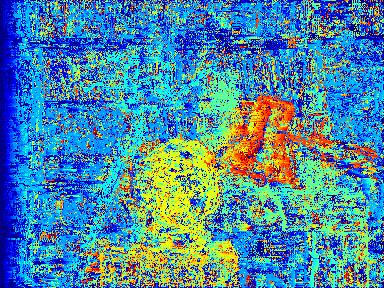
\includegraphics[height=10em]{code/outputs/prob2a.jpg}
  \caption{Unsmoothed disparity map}
\end{figure*}

\spart{b}

\begin{figure*}[!h]
  \centering
  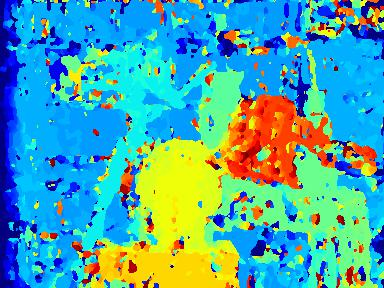
\includegraphics[height=10em]{code/outputs/prob2b.jpg}
  \caption{Disparity map smoothed with bilateral filtering}
\end{figure*}

\solution{3}

\spart{a}

\begin{figure*}[!h]
  \centering
  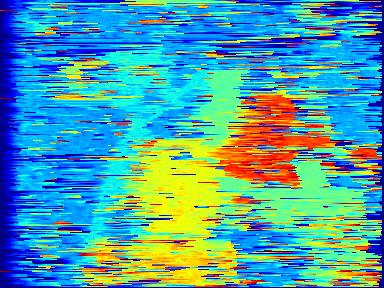
\includegraphics[height=10em]{code/outputs/prob3a.jpg}
  \caption{Left-to-right viterbi output}
\end{figure*}

\spart{b}

\begin{figure*}[!h]
  \centering
  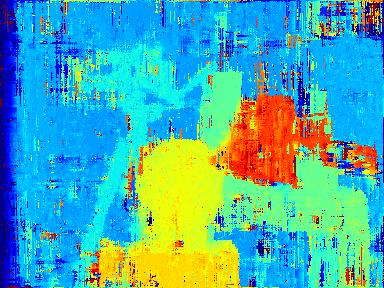
\includegraphics[height=10em]{code/outputs/prob3b.jpg}
  \caption{SGM output}
\end{figure*}

\solution{4}

\begin{figure*}[!h]
  \centering
  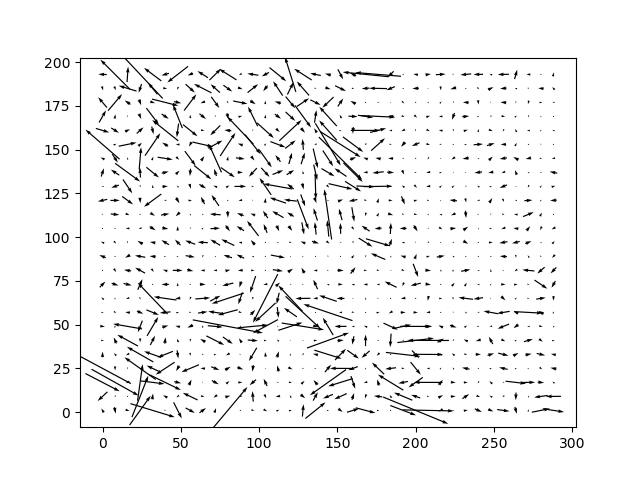
\includegraphics[width=\textwidth]{code/outputs/prob4.png}
  \caption{Optical flow map}
\end{figure*}

\info

This problem set took approximately 16 hours of effort.


I discussed this problem set with:
\begin{itemize}
\item Robbie Derber
\item TAs
\end{itemize}


% Note that you might have to escape some special symbols in URLS like \_
I also got hints from the following sources:
\begin{itemize}
\item The Hirschmuller paper on SGM: http://ieeexplore.ieee.org/stamp/stamp.jsp?arnumber=4359315
\end{itemize}

\end{document}
\grid
